\documentclass[UTF8,openany,zihao=5]{ctexbook}

% 论文版面要求:
% 统一按 word 格式A4纸(页面设置按word默认值)编排、打印、制作。
% 正文内容字体为宋体;字号为小4号;字符间距为标准;行距为25磅(约0.88175cm)。

%%%%% ===== 页面设置
\usepackage[a4paper,top=3cm,bottom=3cm,left=2.5cm,right=2.5cm,%
            ]{geometry}
            

            \usepackage{booktabs}
\usepackage{bicaption}
\captionsetup[figure][bi-first]{name=图}
\captionsetup[figure][bi-second]{name=Fig.}
            
\captionsetup[table][bi-first]{name=表}
\captionsetup[table][bi-second]{name=Tab.}


\usepackage{enumitem}
\setlength{\parindent}{2em}
%默认的弹性间距会导致文中某些排版flush的时候,出现大量空白。
\setlength{\parskip}{0.5em} %指定固定段后间距,默认为弹性间距。
\setlength{\intextsep}{10pt} %固定浮浮动体前后间距。

\ctexset{chapter/break={}}
%%%%% =====章节 标题 设置
\ctexset{%
  contentsname={\vspace{-3.5em}\centerline{\zihao{-3}\heiti 目\quad 录}\vspace{-0.7em}},
  listfigurename={\vspace{-3.5em}\centerline{\zihao{-3}\heiti 插\ 图\ 目\ 录}\vspace{-0.5em}},
  listtablename={\vspace{-3.5em}\centerline{\zihao{-3}\heiti 表\ 格\ 目\ 录}\vspace{-0.5em}},
  bibname={\vspace{-3em}{\zihao{-3}\heiti 参考文献}\vspace{3em}},
%   chapter={
%     name={第,章},
%            number=\chinese{chapter}, %指定章序号为一二三。。。。
%            nameformat={\zihao{3}\bfseries},
%            titleformat={\zihao{3}\bfseries},
%            beforeskip={-10pt},
%            afterskip={20pt}
%            },
  chapter={
            name={,},
            number=\arabic{chapter},
            % number=\arabic{chapter},
            format=\raggedright,
           nameformat={\zihao{3}\bfseries},
           titleformat={\zihao{3}\bfseries},
%           afterskip={1ex plus 0.2ex}
           beforeskip={10pt},% 固定段前段后间距,
           afterskip={5pt}
           },
  section={format=\raggedright,
           nameformat={\zihao{4}\bfseries},
           titleformat={\zihao{4}\bfseries},
%           afterskip={1ex plus 0.2ex}
           beforeskip={1ex},% 固定段前段后间距,
           afterskip={1ex}
           },
  subsection={format=\raggedright,
           nameformat={\zihao{-4}\bfseries},
           titleformat={\zihao{-4}\bfseries},
%           afterskip={0.5ex plus 0.1ex}
           beforeskip={0.5ex},
           afterskip={0.5ex}
           }
}
%%%%% ===== 中英文字体
\setmainfont{Times New Roman}
%\setsansfont{Myriad Pro} % 无衬线字体 sans serif \sffamily
%\setmonofont{Consolas}   % 等宽字体 typewriter \ttfamily
%\newcommand{\Times}{\fontspec{Times New Roman}}
%% 中文字体
%\setCJKmainfont[BoldFont={Microsoft YaHei},ItalicFont={KaiTi}]{NSimSun}
%\setCJKsansfont{Microsoft YaHei}
%\setCJKmonofont{KaiTi}
%\setCJKfamilyfont{STSong}{方正小标宋_GBK}\newcommand{\STSong}{\CJKfamily{STSong}}
\setCJKfamilyfont{songti}{STZhongsong}\newcommand{\STSong}{\CJKfamily{STSong}}

%%%%% ===== 常用宏包
\usepackage{amsmath,amssymb,amsfonts,bm}
\usepackage[amsmath,thref,thmmarks,hyperref]{ntheorem}
\usepackage{graphicx,xcolor,float}
\usepackage{fancyhdr}
\usepackage{tocloft} % 设置目录中的条目间距


\renewcommand\cftdot{\textsubscript{……}}
\renewcommand\cftdotsep{0}

\setlength{\cftbeforechapskip}{1pt}
\renewcommand{\cftchapleader}{\cftdotfill{\cdot}}


\usepackage{booktabs} % toprule, midrule, bottomrule
\usepackage{varwidth} % 可变宽度的 parbox

%%%%% ===== 参考文献与链接
\usepackage[numbers,sort&compress,sectionbib,super, square]{natbib} %引用上标,禁用连续缩写。
\newcommand{\upcite}[1]{\textsuperscript{\cite{#1}}}


\usepackage[xetex,pagebackref]{hyperref}
\hypersetup{CJKbookmarks=true,colorlinks=true,citecolor=blue,%
            linkcolor=blue,urlcolor=blue,bookmarksnumbered=true,%
	        bookmarksopen=true,breaklinks=true}
	        
	        
	        
\iffalse   % 调试时,可去掉,以用于显示引用位置。
\renewcommand*{\backrefalt}[4]{%
\ifcase #1 No citations.%
\or Cited on page #2.%
\else Cited on pages #2.%
%\else #1 Cited on pages #2.%
\fi
}

\else
\renewcommand*{\backrefalt}[4]{}
\fi

%%%%% ===== 浮动图表的标题
% \usepackage[margin=2em,labelsep=space,skip=0.5em,font=normalfont]{caption}
\DeclareCaptionFormat{mycaption}{{\zihao{-5}\heiti\color{blue} #1}#2{\zihao{-5}\kaishu #3}}
\captionsetup{format=mycaption,tablewithin=chapter,figurewithin=chapter}%,belowskip=-10pt
%\setlength{\belowcaptionskip}{-10pt}

%%%%%% ===== 浮动图表的比例默认50%以下,否则无法浮动。
\renewcommand\floatpagefraction{.9} %当浮动体小于页面90%时进行直接放置。
\renewcommand\topfraction{.9}  
\renewcommand\bottomfraction{.9}  
\renewcommand\textfraction{.1}



%%%%% ===== 算法
\usepackage{algorithm,algpseudocode}

%%%%% ===== 其他
\usepackage{ulem}
\def\ULthickness{1pt}




%%%%%===== Code Style代码
\usepackage{listings}
\usepackage{color}

\definecolor{dkgreen}{rgb}{0,0.6,0}
\definecolor{gray}{rgb}{0.5,0.5,0.5}
\definecolor{mauve}{rgb}{0.58,0,0.82}

\lstset{
  language=Python,
  xleftmargin = 3em,xrightmargin = 3em, aboveskip = 1em,
  aboveskip=3mm,
  belowskip=3mm,
  showstringspaces=false,
  columns=flexible,
  rulesepcolor= \color{gray},
  frame = ltrb,
  basicstyle={\normalsize\ttfamily},
  numbers=none,
  numberstyle=\tiny\color{gray},
  keywordstyle=\color{blue},
  commentstyle=\color{dkgreen},
  stringstyle=\color{mauve},
  breaklines=true,
  breakatwhitespace=true,
  tabsize=3
}


\newcommand{\mcc}[1]{\multicolumn{1}{c}{\underline{\makebox[10em][c]{#1}}}}
\newcommand{\mce}[1]{\multicolumn{1}{c}{\underline{\makebox[15em][l]{#1}}}}


\pagestyle{plain}
\fancyhf{}  % 清除以前对页眉页脚的设置

% \newcommand{\makeheadrule}{%% 定义页眉与正文间双隔线
%     \makebox[0pt][l]{\rule[.7\baselineskip]{\headwidth}{0.3pt}}%0.4
%     \rule[0.85\baselineskip]{\headwidth}{1.0pt}\vskip-.8\baselineskip}
% \makeatletter
% \renewcommand{\headrule}{%
%     % {\if@fancyplain\let\headrulewidth\plainheadrulewidth\fi\makeheadrule}}
%     {\makeheadrule}}
% \makeatother
% \renewcommand{\chaptermark}[1]{\markboth{\CTEXthechapter \ #1}{}}
% \renewcommand{\sectionmark}[1]{\markright{\thesection \ #1}{}}
%\fancyhead[RO,LE]{{\small\songti\rightmark}}     % 节标题
%\fancyhead[RE]{{\small\songti\leftmark}}      % 章标题
% \fancyhead[L]{《人工智能的数学思维》课程报告}
% \fancyhead[R]{矩阵运算与网页排名}
% \fancyhead[RO,LE]{$\cdot$ {\small\thepage} $\cdot$}
\fancyfoot[C]{{-\thepage-}}
%\fancyfoot[CO,CE]{{\thepage}}



\begin{document}
\setcounter{page}{1}

\begin{center}
  % \begin{figure}[H]
  %     \vspace{5cm}
  %     
\includegraphics[width=14cm]{images/ecnu.png}
  % \end{figure}
  ~\\[1em]
  {
  \heiti\zihao{-2}{从NP完全问题浅谈计算机系统的局限性}\\
  \zihao{-5}{A Brief Discussion on the Limitations of Computer Systems from NP-Complete Problems}\\
  \vspace{0.8em}
  \kaishu\zihao{4}李鹏达\footnote{李鹏达,2004年4月生,男,华东师范大学软件工程学院本科在读}\\
  \vspace{0.2em}
  \songti\zihao{6}{(10225101460\quad 信息学部\quad 软件工程学院)}
  }
\end{center}

\pagestyle{plain}

% ~\\[1pt]

% \centerline{\zihao{-3}\heiti \textbf{摘\quad 要}}
% \addcontentsline{toc}{chapter}{摘\quad 要}
\linespread{1.1}
{
  \noindent{\zihao{-5} \heiti \textbf{摘\quad 要\quad}}
  \zihao{-5}
  计算机系统是人类创造的最强大的工具之一,它能够高效地执行各种各样的任务,从简单的数学运算到复杂的人工智能。然而,计算机系统并不是万能的,其也存在一些局限性和困难。在计算理论中,有一类特殊的问题被称为NP完全问题(Nondeterministic Polynomial Complete Problem),它们是一类在多项式时间内无法确定是否存在解的问题,而且所有的NP问题都可以在多项式时间内归约到它们。NP完全问题是计算理论中最重要和最困难的问题之一,它们对于理解计算机系统的局限性有重要意义。本文旨在通过介绍NP完全问题的概念、例子、求解方法、应用和价值,浅谈计算机系统在处理一些复杂问题时所面临的局限性和挑战。

  \noindent {\zihao{-5} \heiti \textbf{关键词\quad}}
  \zihao{-5}
  NP完全问题;计算机系统的局限性
}
\linespread{1.25}

\songti\zihao{5}
\chapter{引言}

计算机系统的快速发展使得我们能够处理大规模的数据和执行复杂的任务。从早期的巨型计算机到今天的个人电脑和移动设备,计算机技术已经成为现代社会的核心驱动力。然而,随着计算能力的提高,我们也意识到一些问题是无法在合理的时间内解决的。这些问题被称为NP完全问题,它们是一类计算上困难的问题,涵盖了许多实际生活和计算领域中的重要挑战。

计算机科学领域的研究者们一直致力于寻找高效的算法来解决各种问题。他们发展了各种算法和数据结构,并不断改进计算机系统的性能和效率。然而,随着问题的复杂性增加,我们逐渐认识到存在一些问题,即使在拥有最先进计算机系统的情况下,也无法在可接受的时间内得到准确解答。随着我们用更强大的计算能力和更聪明的算法解决更大和更复杂的问题,这些问题更加显现出来。NP完全性理论可以帮助我们理解这些局限性,P与NP问题开始不仅作为计算机科学中一个有趣的理论问题,而且作为一个基本原理渗透到所有的科学中。\cite{bi:FL}这些问题的存在给计算机系统的发展带来了巨大的挑战,迫使我们重新思考计算的本质和局限性。

在这样的背景下,NP完全问题的概念应运而生。NP完全问题作为计算理论中的一个重要概念,揭示了一类问题的困难性和计算复杂性。它们被证明是计算上最具挑战性的问题之一,其解决方案的计算时间随问题规模的增加呈指数级增长。换句话说,随着问题规模的增大,需要的计算资源呈爆炸式增长,使得这些问题在实际应用中变得不可行。

NP完全问题的定义和特点源于理论计算机科学中的复杂性理论研究。在本文中,我们将从NP完全问题的角度,探讨计算机系统的局限性,并讨论其对计算机科学和现实世界的影响。通过深入研究和分析,我们可以更好地理解NP完全问题对计算机系统的限制,并探索如何应对这些限制,以推动计算机科学的进一步发展。

接下来的章节将介绍NP完全问题的定义和特点,探讨其对计算机系统的局限性,以及在应用和影响方面的重要性。我们将探讨NP完全问题对计算机系统求解能力的限制,以及它们对计算资源的消耗和计算效率的影响。此外,我们还将讨论NP完全问题在密码学、人工智能、运筹学等领域的应用,并探索如何通过近似算法、启发式算法等方法来解决这些问题。最后,我们将讨论克服NP完全问题带来的挑战,并展望未来可能的解决方向。通过对这些问题的深入研究,我们将更好地了解计算机系统的局限性,为未来的研究和发展提供有益的指导,以实现更高效、更可靠的计算系统。

\chapter{NP完全问题简介}



\section{P问题、NP问题与NP难问题}

为了理解NP完全问题,我们首先需要了解P问题、NP问题与NP难问题的概念。
\subsection{P问题}
P问题(P problems)是指可以在多项式时间内解决的问题。在计算复杂性理论中,P类是一类计算问题的集合,这些问题可以由确定性图灵机在多项式时间内有效地求解。
具体而言,一个问题被称为P问题,如果存在一个确定性图灵机算法可以在多项式时间内解决该问题。换句话说,问题的解决方案的运行时间与问题规模成多项式关系。
P类问题具有高效的解决算法,因为它们可以在多项式时间内解决。
\subsection{NP问题}
NP问题是随着计算复杂性理论的产生而出
现的。根据计算复杂性理论,所有科学问题按其解
决时间可分为三大类:多项式类、指数类和不可解
类。但要确定某个具体的问题到底属于哪一类,往
往并非一件容易的事情,尤其是对少数难度大的问
题。\cite{bi:DCF}

NP是"非确定性多项式时间"(Non-deterministic Polynomial-time)的缩写。对于一个问题,如果给定一个候选解,我们可以在多项式时间内验证该解的正确性,那这个问题就被称为NP问题。换句话说,对于一个NP问题,我们可以非确定性地猜测一个解,并在多项式时间内验证该解是否正确。

\subsection{NP难问题}
NP难问题(NP-hard problems)是指在非确定性多项式时间内无法解决的问题。这些问题是计算复杂性理论中的一类,它们不一定属于NP类,但可以被任何一个NP问题在多项式时间内约化到。换句话说,如果我们能够在多项式时间内解决一个NP难问题,那么我们可以在多项式时间内解决所有的NP问题。

具体而言,一个问题被称为NP难问题,如果它满足以下条件:
\begin{enumerate}[noitemsep]
  \item 任何一个NP问题都可以在多项式时间内约化到该问题。也就是说,如果我们能够在多项式时间内解决该问题,那么我们也可以在多项式时间内解决所有的NP问题。
  \item NP难问题不一定属于NP类。虽然NP类中的问题可以在多项式时间内验证解,但NP难问题本身不一定可以在多项式时间内解决。
\end{enumerate}

因此,可以将NP难问题视为计算上的困难问题,其解决方案在一般情况下需要指数级的时间复杂度。需要注意的是,NP难问题是一个相对的概念,即与已知的NP问题相比,它们更难解决。然而,尚未找到证据来证明NP难问题是否可以在多项式时间内解决。

\section{NP完全问题的定义}

NP完全问题是一类特殊的NP问题,具有特殊的性质。一个问题如果满足以下两个条件,就可以被称为NP完全问题。

\begin{enumerate}[noitemsep]
  \item 该问题属于NP类,即给定一个候选解,我们可以在多项式时间内验证该解的正确性。
  \item 该问题是NP难问题,即任何一个属于NP类的问题都可以在多项式时间内约化到该问题。
\end{enumerate}

简单来说,一个问题是NP完全问题,意味着它既是一个NP问题,又是NP难问题。如果我们能够在多项式时间内解决一个NP完全问题,那么我们可以在多项式时间内解决所有的NP问题,因为它们可以通过约化转换为NP完全问题。

研究NP完全问题的一个关键问题是P与NP问题($P=NP$)的探讨。如果能够找到一个多项式时间算法来解决任何一个NP完全问题,那么意味着$P=NP$,即所有的NP问题可以在多项式时间内解决。然而,目前尚未找到证据来证明$P=NP$或$P\ne NP$,这仍然是计算机科学中一个重要的未解决问题。
\vspace{10pt}
\begin{figure}[H]
  \begin{center}
    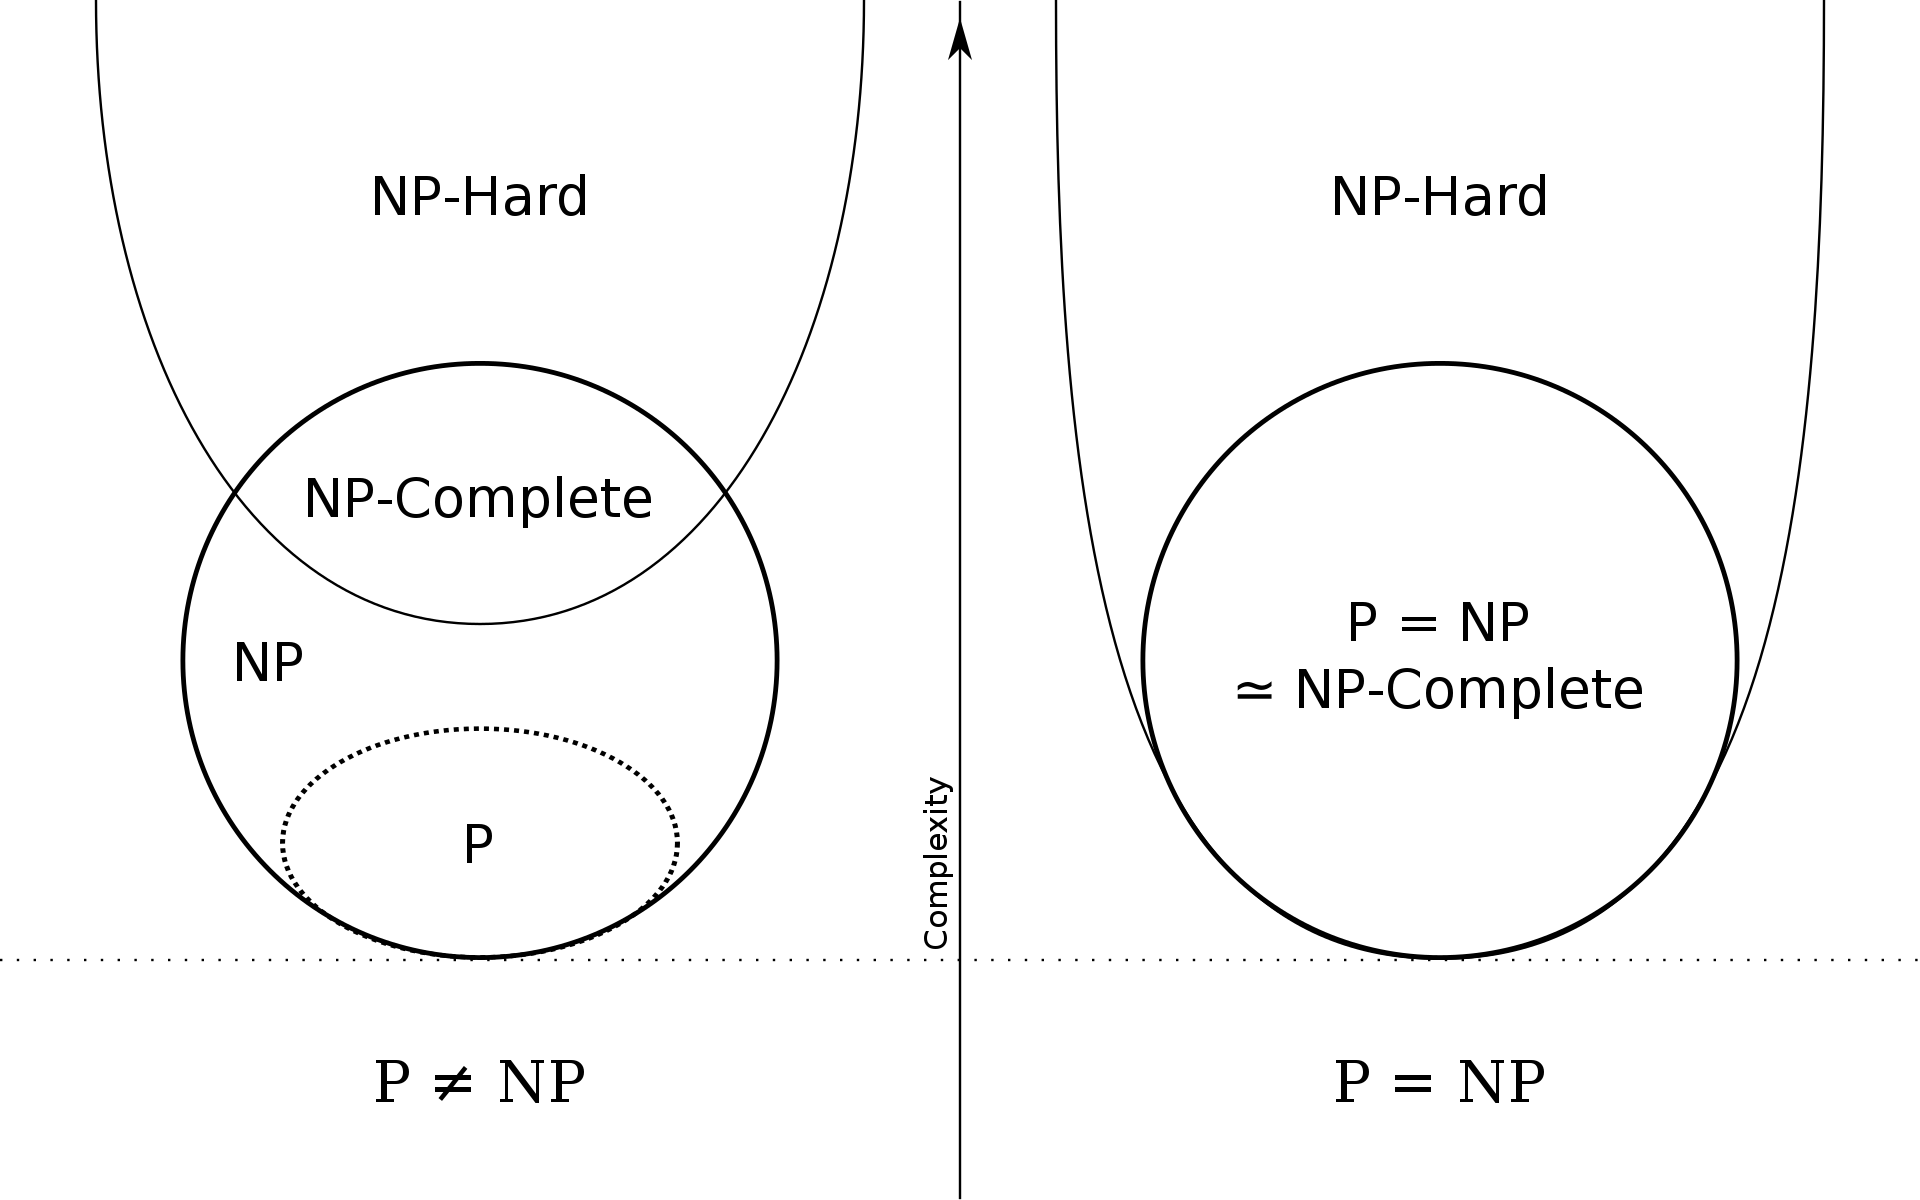
\includegraphics[width=0.3\textwidth]{images/P_np_np-complete_np-hard.svg.png}
    \centering
    \bicaption{描述P问题、NP问题、NP难问题与NP完全问题的欧拉图}{Euler diagram for P, NP, NP-complete, and NP-hard sets of problems}
  \end{center}
\end{figure}

\section{NP完全问题的特点}

由于其特殊性,NP完全问题具有以下几个重要特点:

\begin{enumerate}
  \item 难以在多项式时间内求解:NP完全问题是NP类中最困难的问题之一。虽然可以在多项式时间内验证其解,但尚未找到有效的确定性算法,能够在多项式时间内找到问题的解。这意味着在一般情况下,解决NP完全问题的运行时间随着问题规模的增加呈指数级增长,导致其求解变得非常耗时。
  \item 多项式时间约化:NP完全问题具有多项式时间约化的特性。这意味着任何一个NP问题都可以在多项式时间内转换成NP完全问题。如果我们能够在多项式时间内解决一个NP完全问题,那么根据多项式时间约化的性质,我们也可以在多项式时间内解决所有的NP问题。这种特性使得NP完全问题在NP类中具有特殊的地位。
  \item 具有普适性:NP完全问题的解决对其他NP问题具有普适性。如果我们能够在多项式时间内找到一个解决NP完全问题的算法,那么我们可以将这个算法应用于任何其他NP问题,并在多项式时间内得到其解。这是因为NP完全问题可以在多项式时间内约化到任何其他NP问题,从而证明了其解决方案的普适性。
  \item 问题的多样性:NP完全问题涵盖了多种不同类型的计算问题,包括图论问题、布尔逻辑问题、组合优化问题等。著名的NP完全问题有旅行商问题(TSP)、布尔满足问题(SAT)、子集和问题(Subset Sum Problem)等\cite{bi:KRM}。这些问题的多样性使得NP完全问题的研究对计算机科学的许多领域都具有重要意义。
  \item P与NP问题的关联:NP完全问题与P与NP问题密切相关。如果能够找到一个多项式时间算法来解决任何一个NP完全问题,那么意味着$P=NP$,即所有的NP问题可以在多项式时间内解决。但目前尚未找到证据来证明$P=NP$或$P\ne NP$,这使得NP完全问题的研究成为计算机科学中一个重要的未解决问题。
\end{enumerate}

\section{NP完全问题实例:$N$皇后问题}

$N$皇后问题是一个经典的组合优化问题,最初由欧拉在18世纪提出,并在19世纪得到了广泛研究。问题的目标是在一个$N \times N$的棋盘上放置$N$个皇后,使得它们互相之间不能相互攻击。皇后的攻击范围包括同一行、同一列和同一对角线上的其他皇后。
$N$皇后问题的挑战在于找到一种合法的皇后放置方式,即没有任何两个皇后互相攻击。这要求每行、每列和每条对角线上只能有一个皇后。

\begin{figure}[H]
  \begin{center}
    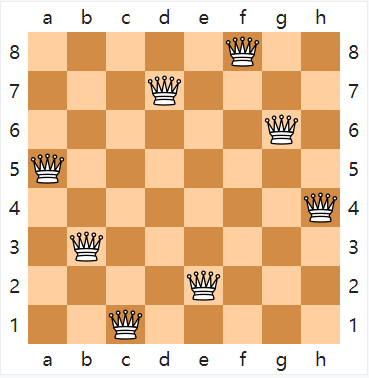
\includegraphics[width=0.3\textwidth]{images/Chessboard480.svg.png}
    \centering
    \bicaption{八皇后问题的唯一对称解}{The only symmetrical solution to the eight queens puzzle}
  \end{center}
  \vspace{-10pt}
\end{figure}

解决$N$皇后问题的常见方法之一是使用回溯算法,也称为深度优先搜索。回溯算法通过递归地尝试所有可能的皇后放置方式,并剪枝以避免无效的路径。具体来说,从第一行开始,对于每一行,尝试将皇后放置在不同的列上。如果当前放置合法,则继续到下一行;如果当前放置导致冲突,则回溯到上一行并尝试下一个列。重复这个过程,直到找到一个合法的解或穷尽所有可能。
\zihao{-5}{
  \begin{table}[H]
    \centering
    \begin{tabular}{cccc}
      \toprule
      序号 & 皇后数量($N$) & 运行结果 & 运行时间 \\
      \midrule
      1    & 2               & 2        & 0ms      \\
      2    & 8               & 92       & 5ms      \\
      3    & 10              & 724      & 45ms     \\
      4    & 12              & 41200    & 2494ms   \\
      4    & 15              & 2279184  & 508649ms \\
      \bottomrule
    \end{tabular}
    \bicaption{解决$N$皇后问题所用的时间}{The time required to solve the N-Queens problem.}
  \end{table}
}
\zihao{5}

尽管回溯算法可以找到$N$皇后问题的解,但在一般情况下,它的时间复杂度非常高。从上表可以看出,随着$N$的增大,计算所用时间迅速加长。对于较大的$N$,回溯算法需要遍历庞大的搜索空间,导致指数级的计算时间。因此,当$N$增大时,$N$皇后问题变得更加困难。

$N$皇后问题不仅在计算机科学领域中受到广泛关注,还在数学、人工智能和教育领域中具有重要的研究价值。它被用作算法设计和计算复杂性理论的典型案例,帮助人们理解组合优化问题的本质和解决方法\cite{bi:XZL}。







\chapter{NP完全问题的局限性}

\section{快速求解的困难性}

NP完全问题的一个显著特点是在多项式时间内快速求解它们的困难性。尽管我们可以在多项式时间内验证一个解的正确性,但找到一个解却是一个耗时的任务。这就意味着对于大多数NP完全问题,我们无法找到一种高效的算法来解决它们。

为了更好地理解快速求解的困难性,让我们以一个具体的NP完全问题——旅行商问题(Traveling Salesman Problem,TSP)为例。TSP要求在给定的一组城市之间找到一条最短路径,使得每个城市都被恰好访问一次,最后返回出发城市。其在图论中的一个等价问题为:给定一个加权完全图(顶点表示城市,边表示道路,权重就会是道路的成本或距离), 求一权值最小的哈密尔顿回路。

\vspace{10pt}
\begin{figure}[H]
  \begin{center}
    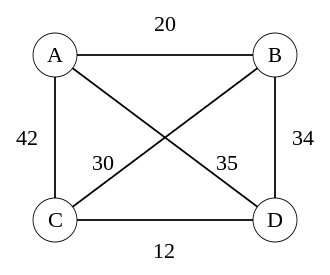
\includegraphics[width=0.35\textwidth]{images/Weighted_K4.svg.png}
    \centering
    \bicaption{四个城市的对称旅行商问题}{Symmetric TSP with four cities}
  \end{center}
\end{figure}

TSP的解法包括穷举法、贪婪算法、最近邻算法、2-近似算法等。穷举法尝试列举所有可能的路径,但在大规模问题上不实用。贪婪算法和最近邻算法是基于局部最优选择的启发式方法,它们通过逐步选择最近的未访问城市来构建路径。2-近似算法基于最小生成树构建哈密顿回路,可获得路径长度不超过最优解的两倍。除了这些方法,还有其他启发式算法和元启发式算法可用于解决TSP问题,如遗传算法、模拟退火算法和禁忌搜索等\cite{bi:STV}。这些算法通过利用问题特性和结构,以近似的方式搜索解空间,寻找接近最优解的解。

然而,TSP是一个典型的NP完全问题,其求解的时间复杂度是指数级的。随着城市数量的增加,解决TSP问题所需的时间呈现出指数级的增长。事实上,对于较大规模的城市集合,即使使用当前最好的算法和计算资源,找到最优解也是一项几乎不可能完成的任务。

这种快速求解的困难性对算法设计和计算机系统的开发产生了重大影响。它限制了我们在某些实际问题中的求解能力,特别是那些涉及大规模数据和复杂约束的问题。对于许多现实世界的优化、调度、路径规划和布局问题等,很难找到有效的算法来在合理的时间内得到最优解。

尽管存在一些近似算法和启发式方法来解决NP完全问题,它们通常只能提供接近最优解的近似结果,并不能保证找到确切的最优解。因此,在实际应用中,我们必须在解决NP完全问题的精确性和求解时间之间进行权衡,并选择合适的方法来满足问题的需求和限制。

综上所述,NP完全问题的快速求解困难性对计算机系统的性能和效率产生了重大影响。在解决NP完全问题时,我们必须认识到其困难性,并寻求创新的算法设计和资源管理策略,以在实际应用中找到可行的解决方案。

\section{计算资源消耗}

在计算资源消耗方面,NP完全问题给计算机系统带来了显著的挑战。这些问题的困难性质导致了解决它们所需的计算资源大幅增加。在本节中,我们将详细探讨这些问题对计算资源的消耗以及相关的局限性。

首先,由于NP完全问题的解空间非常庞大,求解这些问题通常需要进行全面的搜索。穷举所有可能的解是一个非常耗时的过程,特别是对于具有大规模问题的情况。搜索空间的大小随着问题规模的增加呈指数级增长,使得在有限的时间内找到最优解或近似最优解变得非常困难。这就需要大量的计算资源和时间来进行计算。

其次,许多解决NP完全问题的算法在最坏情况下的时间复杂度是指数级的。例如,穷举法需要对所有可能的解进行逐个验证,其时间复杂度是$O(n!)$,其中$n$是问题的规模。即使是一些相对高效的启发式算法和近似算法,其时间复杂度仍然与问题规模成正比。这使得处理大规模问题变得非常困难,并且可能需要非常长的时间才能获得可接受的解。

此外,NP完全问题的计算资源消耗还受限于计算机系统的存储资源。在搜索和计算过程中,需要存储和操作大量的数据结构,例如问题的输入数据、中间结果和候选解。对于具有大规模问题的情况,存储这些数据可能需要大量的内存空间,而计算机系统的存储能力可能是有限的。这进一步增加了解决NP完全问题的挑战,因为系统必须能够有效地管理和利用存储资源。

另一个重要的考虑因素是NP完全问题对计算系统的扩展性和可伸缩性提出了挑战。当问题规模增加时,需要更多的计算资源来处理更大规模的数据和计算任务。这要求计算机系统具备良好的可扩展性,能够有效地分配和利用计算资源。然而,由于NP完全问题的计算资源消耗较高,系统的可扩展性可能受到限制,特别是在资源受限的环境下。

NP完全问题的困难性质对计算机系统的计算资源消耗带来了显著的影响。解决这些问题需要大量的计算资源和时间,并且可能受限于存储资源和系统的可扩展性\cite{bi:AB}。为了克服这些限制,研究人员一直在努力寻找更高效的算法和方法,以降低计算资源的消耗,并提高计算机系统的性能和可伸缩性。

\section{对密码学和安全性的影响}
由于NP完全问题的困难性质,它们对密码学和安全性产生了重要的影响和挑战。

首先,许多加密算法和安全协议的设计是基于NP完全问题的困难性假设。这些算法和协议利用了NP完全问题的解空间庞大和计算资源消耗高的特性,以保证其安全性。例如,公钥加密算法如RSA和椭圆曲线密码学中的离散对数问题以及RSA中的因子分解问题,都基于NP完全问题的困难性假设。如果这些NP完全问题能够在多项式时间内解决,那么整个密码学体系将遭受重大威胁。

其次,NP完全问题的困难性也与密码分析密切相关。密码分析是研究破解密码算法和协议的方法和技术。如果NP完全问题能够在多项式时间内解决,那么攻击者可能能够通过求解这些问题来破解密码算法和协议。因此,NP完全问题的困难性保证了密码算法和协议的安全性,提供了对抗密码分析的基础。

此外,NP完全问题的困难性还对密码学中的其他方面产生了影响。例如,密码学中的零知识证明和密码编码等技术也依赖于NP完全问题的困难性假设。这些技术的安全性建立在NP完全问题的难解性上,以保证信息的机密性和完整性。

需要注意的是,尽管NP完全问题的困难性提供了密码学安全性的基础,但它并不能证明密码学的绝对安全性。由于P与NP问题的未解决性,我们无法确定是否存在多项式时间的算法来解决NP完全问题。因此,虽然NP完全问题的困难性假设被广泛接受,但仍存在一定的不确定性。

综上所述,NP完全问题对密码学和安全性产生了重要的影响。它们为密码算法和协议的设计提供了基础,并提供了对抗密码分析的保障。然而,我们仍然需要不断研究和发展更强大的密码算法和安全协议,以应对未来可能的攻击和突破。

\chapter{NP完全问题的应用与策略}

NP完全问题在计算机科学领域中具有广泛的应用和重要的影响。尽管这些问题的解决具有困难性,但它们对许多实际应用和理论研究产生了深远的影响。本节将详细介绍NP完全问题的应用领域以及它们对这些领域的影响。

首先,NP完全问题在运筹学和优化问题中扮演着重要角色。运筹学是研究如何在给定约束条件下寻找最优解的学科。许多经典的运筹学问题,如旅行商问题、背包问题和图着色问题,都被证明是NP完全问题。尽管在多项式时间内解决这些问题是困难的,但近似算法和启发式算法被广泛应用于寻找接近最优解的解决方案。这些方法在实际应用中用于资源分配、路径规划、排产等问题,为实际决策提供了有效的工具。例如,在物流领域中,通过使用启发式算法解决旅行商问题,可以优化货物的配送路径,减少成本和时间。

其次,NP完全问题在人工智能和机器学习领域中具有重要意义。在图像识别、自然语言处理、数据挖掘等任务中,我们经常需要在大规模数据集中寻找最佳解决方案。这些搜索问题可以被建模为NP完全问题,如最小生成树问题和布尔可满足性问题。虽然准确解决这些问题的计算复杂度很高,但通过使用启发式搜索算法、进化算法和深度学习等技术,我们能够获得近似解或高效的解决方案。这些方法在图像处理、自然语言处理和数据挖掘等领域取得了重要的应用和突破\cite{bi:PAL}。例如,在图像处理中,通过使用近似算法解决图像分割问题,可以实现对图像中不同对象的精确提取。

此外,NP完全问题的研究也推动了计算理论的发展\cite{bi:BK}。研究人员提出了许多与NP完全问题相关的理论和概念,如多项式时间可约化、近似算法和参数化复杂性等。这些理论的发展不仅帮助我们更好地理解NP完全问题的本质和限制,还为其他计算问题的分析和解决提供了基础。例如,近似算法的设计原理和参数化复杂性的研究方法,不仅适用于NP完全问题,也可以应用于其他计算问题的优化和近似求解。

总结起来,尽管NP完全问题的解决具有困难性,但它们在运筹学、人工智能、机器学习和计算理论等领域中具有广泛的应用和重要的影响。通过使用近似算法、启发式算法和优化技术,我们能够获得接近最优解的结果,为实际问题提供了有效的解决方案。此外,NP完全问题的研究也推动了计算理论的发展,促使人们思考计算复杂性的本质和界限。对于实际应用和理论研究而言,了解和解决NP完全问题的困难性具有重要意义。

\chapter{应对NP完全问题的挑战}

\section{近似算法与启发式算法}

近似算法和启发式算法是在解决NP完全问题时常用的方法,它们可以在合理的时间内找到近似最优解或较好的解决方案。我们将详细介绍这两种算法的基本原理和应用。

近似算法是一种寻找问题的近似最优解的方法,其目标是在可接受的时间内找到一个解决方案,该方案与最优解之间的差距被限制在一定的范围内。近似算法的设计思想是通过权衡计算效率和解决方案质量,以达到在实践中可接受的性能。在设计近似算法时,需要考虑问题的特点和约束条件,以及算法的时间复杂性和近似比等因素。
一种常用的近似算法是贪心算法。贪心算法通过每次选择当前局部最优的解决方案来逐步构建全局解。虽然贪心算法不能保证获得最优解,但它通常可以在多项式时间内找到近似最优解。另一种常见的近似算法是近似比算法,它通过确定一个上界或下界来评估解决方案的质量,并确保找到的解决方案与最优解之间的差距是可接受的。

近似算法在许多实际问题中得到了广泛应用。例如,在旅行商问题中,贪心算法可以通过选择每次最近的未访问城市来构建一个近似最优的旅行路线。在图着色问题中,近似算法可以通过对每个节点分配一个可用的颜色来实现图的着色,使得相邻节点具有不同的颜色。

启发式算法是基于经验和启发性规则的一类搜索算法,用于在大规模问题中寻找较好的解决方案。启发式算法的设计灵感来自于人类的问题解决思维,它通过不完全的搜索和剪枝策略来减少搜索空间,以获得满足要求的解决方案。
启发式算法通常由三个主要组成部分构成:初始解生成、邻域搜索和解评估。初始解生成阶段通过一定的规则或随机性生成一个初始解,作为搜索的起点。邻域搜索阶段根据问题的特点和约束条件,通过改变当前解中的某些部分来生成邻近解,然后通过评估这些邻近解的质量来选择下一步的移动方向。解评估阶段根据问题的目标函数或评价准则,对生成的解进行评估和比较,并选择具有更好性能的解作为当前解。

启发式算法在解决大规模和复杂问题时具有较好的性能。例如,在物流配送问题中,启发式算法可以根据货物的重量、距离和时间窗口等约束条件,通过不断调整路径和车辆分配来优化配送效率。在机器学习中,启发式算法可以通过选择合适的特征子集或调整模型的参数来提高预测准确性。

总之,近似算法和启发式算法是解决NP完全问题的重要方法。它们通过权衡计算效率和解决方案质量,以在可接受的时间内找到较好的解决方案。这些算法在实际问题中具有广泛的应用,并为我们解决复杂问题提供了有效的工具和思路。

\section{并行计算}

并行计算在解决NP完全问题方面发挥着重要作用。由于NP完全问题的困难性,我们通常无法找到多项式时间内的精确解决方案。然而,并行计算提供了一种通过利用多个处理单元并行执行任务来加速求解的方法,从而在实践中克服了部分问题的困难。

并行计算可以在多个层次上应用于解决NP完全问题。首先,任务级并行可以将大规模问题分解为多个子问题,并在多个处理单元上并行执行这些子问题。每个处理单元可以独立地求解其分配的子问题,然后将结果进行合并,从而加快整体求解的速度。这种任务级并行适用于具有明显独立性的NP完全问题,如图论算法中的最短路径问题和旅行商问题等。

其次,数据级并行可以将问题的数据划分为多个块或部分,并在多个处理单元上并行处理这些数据。每个处理单元使用相同的算法和操作来处理不同的数据块,从而实现对整个数据集的并行处理。数据级并行适用于需要对大规模数据集进行相同类型操作的NP完全问题,如图着色问题和布尔满足问题等。

此外,指令级并行也可以应用于解决NP完全问题。现代处理器中的并行指令集、流水线和超标量等技术可以同时执行多个指令,从而提高计算速度。通过将算法和操作优化为适合指令级并行的形式,可以在处理器上实现更高效的NP完全问题求解。

通过并行计算,我们可以利用多个处理单元的计算能力和资源,并通过同时执行多个任务或操作来加快求解速度。这对于NP完全问题的求解具有重要意义,因为它们往往涉及大规模的计算和复杂的搜索空间。并行计算的使用可以提高算法的效率,并使我们能够处理更大规模的问题实例。

然而,并行计算在解决NP完全问题时也面临一些挑战和限制。首先,问题的并行化可能会导致通信和同步的开销。处理单元之间需要进行数据传输和结果合并,这可能会引入额外的计算和通信开销,影响整体的求解效率。其次,并行计算的可扩展性是一个关键问题。随着问题规模的增加,需要更多的处理单元来进行并行计算。然而,并行计算的效率在处理单元数量增加时并不总是线性增长,因此在设计并行算法时需要考虑可扩展性和负载均衡的问题。

\section{量子计算}

量子计算是一种基于量子力学原理的计算模型,与传统的经典计算有所不同。它利用量子比特(qubits)的叠加和纠缠性质,可以在相对较短的时间内处理大规模的计算问题。在解决NP完全问题方面,量子计算被认为具有巨大的潜力和可能性。本节将详细介绍量子计算与NP完全问题之间的关系,以及量子计算在克服这些问题上的应用和影响。

首先,我们知道NP完全问题是指那些可以在多项式时间内验证解答的问题,但尚未找到多项式时间内求解的算法。传统的经典计算模型在解决这些问题时,通常需要进行穷举搜索或使用近似算法来获取接近最优解的结果。然而,量子计算的特殊性质为解决这些问题提供了一种新的可能性。

量子计算通过利用量子叠加和纠缠的特性,可以在一次计算中同时处理多个可能性。相比之下,经典计算必须逐个遍历每个可能的状态,而量子计算可以在同一时间内处理所有可能的状态。这使得量子计算在搜索和优化问题的求解中具有显著的优势。对于NP完全问题,量子计算可以通过量子算法来探索更快速的解决方案。

在量子计算领域,已经提出了一些与NP完全问题相关的量子算法。其中最著名的是Grover搜索算法和量子近似优化算法\cite{bi:GG}(Quantum Approximate Optimization Algorithm,QAOA)。Grover搜索算法通过利用量子并行和干涉的特性,可以在$O(\sqrt{N})$次搜索中找到未排序数据库中的目标项,相比于经典算法的$O(N)$次搜索,具有显著的加速效果。QAOA则通过将问题转化为约束优化问题,并利用量子态的演化过程来搜索最优解\cite{bi:GG}。这些量子算法为解决NP完全问题提供了新的思路和方法。

尽管量子计算在解决NP完全问题方面具有潜力,但实际上,目前的量子计算技术还处于早期阶段,并且面临着许多挑战。目前的量子计算机数量较少,其稳定性和纠错能力仍然是一个难题。此外,量子计算中的量子比特易受噪声和干扰的影响,导致计算结果的误差率较高。这些限制限制了量子计算在实际应用中的规模和准确性。

\chapter{总结:NP完全问题与计算机系统的局限性}

NP完全问题是计算机科学中的一个重要概念,它揭示了计算机系统在某些情况下的困难和局限性。在这个部分中,我们将详细介绍NP完全问题以及与计算机系统的局限性之间的关系。

NP完全问题属于一类特殊的计算问题,其特点是虽然很容易验证一个给定解是否正确,但要在合理的时间内找到一个解却非常困难。这意味着如果一个问题是NP完全问题,那么在目前已知的算法中,没有高效的方法可以解决它。著名的旅行商问题和背包问题就是NP完全问题的例子。

NP完全问题的困难性使得它们在计算机系统中具有重要的局限性。首先,由于NP完全问题的困难性,我们无法找到一种通用算法来解决所有这类问题。换句话说,不存在一种能够在多项式时间内解决所有NP完全问题的算法。这使得在实际应用中,我们需要依赖启发式算法或者近似算法来寻找近似解。虽然这些方法在某些情况下可以提供可行的解决方案,但它们无法保证找到最优解。这就限制了我们对NP完全问题的求解能力。

其次,NP完全问题对计算资源的要求非常高。由于NP完全问题的指数级复杂性,它们的求解时间随着问题规模的增长呈指数级增长。这就意味着当问题规模变大时,求解时间将会变得非常长。在实际应用中,这可能导致我们无法在合理的时间内得到一个可行的解决方案。这也是为什么在现实生活中,我们常常会面临一些问题,即使利用最先进的计算机系统,也很难得到一个满意的解决方案。

此外,NP完全问题的存在性对于计算理论和密码学也具有重要意义。事实上,许多加密算法的安全性基于NP完全问题的困难性。例如,公钥密码学中的因子分解问题被认为是一个NP完全问题,而这个问题的难解性被广泛应用于RSA加密算法。因此,如果NP完全问题可以在多项式时间内解决,那么许多密码学体系将会被破解,导致计算机系统的安全性遭到威胁。

尽管NP完全问题的困难性使得找到确切的最优解变得困难,但仍然可以通过一些技术来进行问题的优化。一种常见的优化方法是启发式算法,通过利用问题的特定性质和启发性的搜索策略来找到接近最优解的解决方案。另一种优化方法是近似算法,通过在可接受的时间范围内找到一个接近最优解的近似解决方案。此外,对NP完全问题进行问题实例特定的优化也是一种常用的策略,通过对问题的特定实例进行深入分析,可以发现某些特殊性质或规律,并基于这些特性设计出更高效的算法。

在计算机系统中,对NP完全问题的优化方法具有重要的应用价值。例如,在路线规划和资源分配等实际问题中,优化旅行商问题和背包问题等NP完全问题的求解效率可以大大提高系统的性能和效率。通过启发式算法、近似算法和问题实例特定的优化,我们可以在可接受的时间内找到接近最优的解决方案。这些优化方法在计算机系统中的应用可以提高系统的性能和效率,并在实际问题中得到广泛应用。因此,虽然NP完全问题的困难性限制了我们找到确切的最优解的能力,但通过这些优化方法,我们能够在实践中找到满足要求的高质量解。

综上所述,NP完全问题在计算机系统中具有重要的局限性。它们的困难性使得我们无法找到高效的算法来解决这类问题,并且对计算资源的要求非常高。此外,NP完全问题的存在性对计算理论和密码学也具有重要的影响。尽管我们可以使用启发式算法和近似算法来寻找可行的解决方案,但在大规模和安全性要求较高的场景下,这些方法可能无法满足需求。因此,对于NP完全问题的研究和理解对于计算机科学的发展和实际应用具有重要意义。

% \newpage
\setlength{\bibsep}{1ex}  % 需 natbib 宏包
\begin{thebibliography}{99}
  \addcontentsline{toc}{chapter}{参考文献}
  \thispagestyle{plain}

  % \addtolength{\itemsep}{-5pt}

  \bibitem{bi:FL}
  Fortnow L. The status of the P versus NP problem[J]. Communications of the ACM, 2009, 52(9): 78-86.

  \bibitem{bi:DCF}
  杜立智, 陈和平, 符海东. NP 完全问题研究及前景剖析[J]. 武汉工程大学学报, 2015, 37(10): 73-78.

  \bibitem{bi:KRM}
  Karp R M. Reducibility among combinatorial problems[M]. Springer Berlin Heidelberg, 2010.

  \bibitem{bi:XZL}
  徐少飞, 张立臣, 李鹏. 一种求解 n 皇后问题的概率回溯复合算法[J]. 现代计算机, 2021.

  \bibitem{bi:STV}
  Svensson O, Tarnawski J, Végh L A. A constant-factor approximation algorithm for the asymmetric traveling salesman problem[J]. Journal of the ACM (JACM), 2020, 67(6): 1-53.

  \bibitem{bi:AB}
  Arora S, Barak B. Computational complexity: a modern approach[M]. Cambridge University Press, 2009.

  \bibitem{bi:PAL}
  Prates M, Avelar P H C, Lemos H, et al. Learning to solve np-complete problems: A graph neural network for decision tsp[C]. Proceedings of the AAAI Conference on Artificial Intelligence. 2019, 33(01): 4731-4738.

  \bibitem{bi:BK}
  Bittel L, Kliesch M. Training variational quantum algorithms is NP-hard[J]. Physical review letters, 2021, 127(12): 120502.

  \bibitem{bi:GG}
  Guerreschi G G, Matsuura A Y. QAOA for Max-Cut requires hundreds of qubits for quantum speed-up[J]. Scientific reports, 2019, 9(1): 6903.
\end{thebibliography}

\end{document}